%----------------------------------------------------------------------------------------
%	PACKAGES AND DOCUMENT CONFIGURATIONS
%----------------------------------------------------------------------------------------

\documentclass{article}

\usepackage[version=3]{mhchem} % Package for chemical equation typesetting
\usepackage{siunitx} % Provides the \SI{}{} and \si{} command for typesetting SI units
\usepackage{graphicx} % Required for the inclusion of images
\usepackage{natbib} % Required to change bibliography style to APA
\usepackage{amsmath} % Required for some math elements
\usepackage[export]{adjustbox}

\setlength\parindent{0pt} % Removes all indentation from paragraphs

\renewcommand{\labelenumi}{\alph{enumi}.} % Make numbering in the enumerate environment by letter rather than number (e.g. section 6)

%\usepackage{times} % Uncomment to use the Times New Roman font

%----------------------------------------------------------------------------------------
%	DOCUMENT INFORMATION
%----------------------------------------------------------------------------------------

\title{Progetto 02 \\ Smart Coffee Machine} % Title

\author{Paolo Baldini \and Andrea Giulianini} % Author name

\date{\today} % Date for the report

\begin{document}

\maketitle % Insert the title, author and date

% If you wish to include an abstract, uncomment the lines below
% \begin{abstract}
% Abstract text
% \end{abstract}

%----------------------------------------------------------------------------------------
%	SECTION 1
%----------------------------------------------------------------------------------------

\section{Specifics}

Si vuole realizzare un sistema embedded che implementa una macchina del caffè smart.
\newline\newline
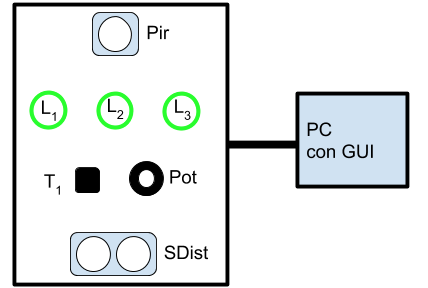
\includegraphics[scale=0.55,center]{res/img/scm.png}

% If you have more than one objective, uncomment the below:
%\begin{description}
%\item[First Objective] \hfill \\
%Objective 1 text
%\item[Second Objective] \hfill \\
%Objective 2 text
%\end{description}

\subsection{Components}

\begin{itemize}
	\item 3 led (L1, L2, L3) verdi
	\item 1 pulsante tattile T1 e 1 potenziometro Pot
	\item 1 sensore di movimento PIR e un sonar SDist
	\item Collegamento seriale con PC
\end{itemize}

\subsection{System Behaviour}

La macchina parte in una modalità STAND BY, in cui si presuppone avere un consumo ridotto di energia elettrica.  Quando viene rilevata la presenza di qualcuno nelle vicinanze allora esce dalla modalità di risparmio, entrando in una modalità ON.
\newline\newline
Se viene rilevato qualcuno  ad una distanza inferiore a DIST1 cm per un certo numero DT1 secondi, viene visualizzato un messaggio “Welcome!” sulla GUI lato PC e la macchina entra in una modalità READY, in cui può accettare comandi.  Se la macchina non rileva più nessuno entro quella distanza per DT2a secondi, la macchina torna nella modalità ON. Dalla modalità ON la macchina torna in modalità STAND BY se non viene rilevata la presenza di nessuno per DT2b secondi.
\newline\newline
In modalità READY, l’utente può regolare lo zucchero con la manopola POT. Ogni volta che cambia il livello di zucchero, lato PC viene visualizzato opportunamente il livello aggiornato di zucchero  (mediante componente grafico o messaggio testuale).
\newline\newline
L’utente può fare un caffè premendo il pulsante T1. Quando preme il pulsante, parte il processo rappresentato dall’accensione progressiva dei 3 led, della durata di DT3 secondi. Lato PC, viene visualizzato il messaggio “Making a coffee”  e poi “The coffee is ready” quando il caffè è pronto.
\newline\newline
L’utente ha tempo DT4 secondi per prendere il caffè - in questo caso si simula con distanza che va sotto i DIST2 cm, ovvero: rilevo distanza sotto DIST2 cm, significa che l’utente ha preso il caffè. Se non si prende il caffè entro DT4 secondi, in ogni caso la macchina torna nella modalità READY (e viene rimosso il messaggio lato PC).
\newline\newline
Infine, la coffee machine può esaurire il materiale per il caffè. Si suppone che possa essere caricata per fare NMAX caffè. Dopo aver fatto NMAX caffè, lato viene prodotto il messaggio “No more coffee. Waiting for recharge” ed entra in modalità MAINTENANCE.  In questa modalità, il sistema aspetta il ricaricamento che può avvenire mediante un’azione lato PC (es: pulsante di ricarica), corrispondente ad una certa quantità di dosi NC. Avvenuta la ricarica, lato PC viene visualizzato il messaggio “Coffee refilled: “+NC e la macchina torna in modalità STAND BY.
\newline\newline
Realizzare il sistema su Arduino + PC collegati via seriale, implementando il programma su Arduino in C++ e il programma su PC in Java.  Utilizzare un approccio a task, con modello di comportamento basato su macchine a stati finiti sincrone.

\subsection{Default Value}
\vskip 0.1 cm
\begin{itemize}
	\item DIST1 (Engagement distance) = 0.3 m
	\item DIST2 (Take coffee) = 0.1 m
	\item DT1 (Min engagement time) = 1 s
	\item DT2a (Max time with no engagement) = 5 s
	\item DT2b (Max time with no presence) = 5 s
	\item DT3 (Coffee making process duration) = 3 s
	\item DT4 (Max time to remove coffee) = 5 s
\end{itemize}
\vskip 0.1 cm
Per tutti gli aspetti non specificati, fare le scelte che si credono più opportune.
\newpage

%----------------------------------------------------------------------------------------
%	SECTION 2
%----------------------------------------------------------------------------------------

\section{Project Solution}
\subsection{Introduction to the Approach}
La soluzione del progetto viene fornita, come richiesto, con l'approccio a task. Ogni task svolge un compito, per quanto semplice esso sia. Anche se alcuni elementi non avrebbero veramente avuto bisogno di un task singolo, ma sarebbero potuti essere inseriti direttamente nelle classi che li utilizzavano (vedi pir), è stato comunque scelto di utilizzare una filosofia di "scorporamento" abbastanza aggressiva per massimizzare la modularità del sistema. Ne risulta un sistema con più entità in gioco di quelle necessarie, ma il funzionamento non risulta affatto più complesso di un sistema con minor modulazione. \newline
I moduli, i task e le entità del progetto dialogano attraverso variabili comuni. Non è stato volontariamente utilizzato il termine "globali" perchè effettivamente globali queste non sono. Queste variabili comuni sono infatti incluse dentro una struttura dati, e non istanziate singolarmente tramite la keyword "extern". Non c'è un vero motivo per il quale abbiamo preferito questo approccio ne abbiamo trovato un motivo per il quale questo possa essere svantaggioso, è stata quindi una pura scelta implementativa.

\subsection{Task Analize}
In questa sezione verrà analizzato l'utilizzo dei singoli task e la logica che vi è dietro. Le FSM verranno mostrate e analizzate in una sezione a se stante posta successivamente a questa.

\subsubsection{Scheduler}
Questo non è un task, ma è l'entità che permette all'approccio a task di avere applicazione. Ogni tot millisecondi esce da un costante stato di sleep per lanciare in esecuzione i vari task. L'uscita dallo stato di sleep è determinata dall'interrupt generato dal watchdog timer (settato come interrupt e non reset).

\subsubsection{ITask}
Non si tratta di un vero e proprio task ma di un interfaccia alla quale questi devono aderire per essere considerati tali. Definisce un metodo virtuale puro Exec() che verrà richiamato dallo scheduler ogni volta che il task dovrà essere eseguito.

\subsubsection{Distance}
Il compito di questo task consiste nel valutare se la distanza acquisità dal sensore di prossimità rientra nel range valutato in uno specifico stato. Se ad esempio ci troviamo nello stato ON, allora sappiamo che la distanza richiesta per passare allo stato READY deve essere inferiore a DIST1. Con questi dati possiamo informare gli altri task (tramite variabili condivise) se un individuo si trova nel "range" corretto per il passaggio al successivo stato.

\subsubsection{MakeCoffee}
Se la macchina si trova nello stato MAKING\_COFFEE, questo si occuperà di "preparare il caffe" e di visualizzare l'avanzamento della preparazione tramite i led. Sarebbe anche stato possibile scomporre la gestione dei led in un ulteriore task (per permetterne la gestione in ulteriori possibili circostanze non specificate nel testo), ma per mancanza di tempo e per la relativa utilità di questo nel contesto attuale si è deciso di integrare le due parti.

\subsubsection{Postman}
Quest'entità si occupa di inviare i messaggi accodati da altri task e di riceverne tramite la seriale. La logica è semplice: se sono presenti messaggi da inviare allora li trasmette, mentre se sono presenti messaggi in arrivo allora li riceve dalla seriale.

\subsubsection{Potentiometer}
Questo task acquisisce il valore del potenziometro e lo mappa nelle varie possibili quantità selezionabili. Se il valore acquisito differisce da quello precedente, allora richiede l'invio di un messaggio attraverso la seriale che notifichi il cambiamento.

\subsubsection{Presence}
E' il task che si occupa di catturare la presenza o assenza di un individuo tramite il sensore a infrarossi. Non sarebbe stato necessario creare un task solo per questo sensore, ma data la sua importanza a livello logico e di gestione nel programma, abbiamo ritenuto che inserirlo come task avrebbe suscitato in un lettore (del codice) un idea lampante di quanto questo elemento sia fondamentale nel funzionamento della macchina.

\subsubsection{StateSwitcher}
E' il task che si occupa del passaggio di stato della macchina. La transizione è definita dalle variabili settate dagli altri task (e.g.: pir\_present).

\subsubsection{Timer}
L'idea dietro al task timer è che a seconda dello stato generale della machina questo dovrà partire (o aspettare in alcuni casi: vedasi stato "READY in range") con l'intento di raggiungere differenti tempistiche. Allo scadere del timer questo notificherà l'evento agli altri stati tramite il solo utilizzo di variabili globali. Questa separazione del compito evita che all'inserimento di un nuovo task si debba andare a inserire all'interno del timer un riferimento a quest'ultimo ed evitando quindi che il timer debba andare a notificare direttamente a questo l'esito.

\newpage
%----------------------------------------------------------------------------------------
%	SECTION 3
%----------------------------------------------------------------------------------------

\section{Finite State Machines - Schemes}
Sono di seguito presentate le macchine a stati finiti relative alle componentistiche più importanti e meno banali del programma. Sono quindi escluse dalla trattazione FSM presentanti solo due stati e con condizioni banali (come può ad esempio risultare quella del sensore di presenza).

\subsection{Overview}
\vskip 0.3 cm
\begin{center}
\centering { 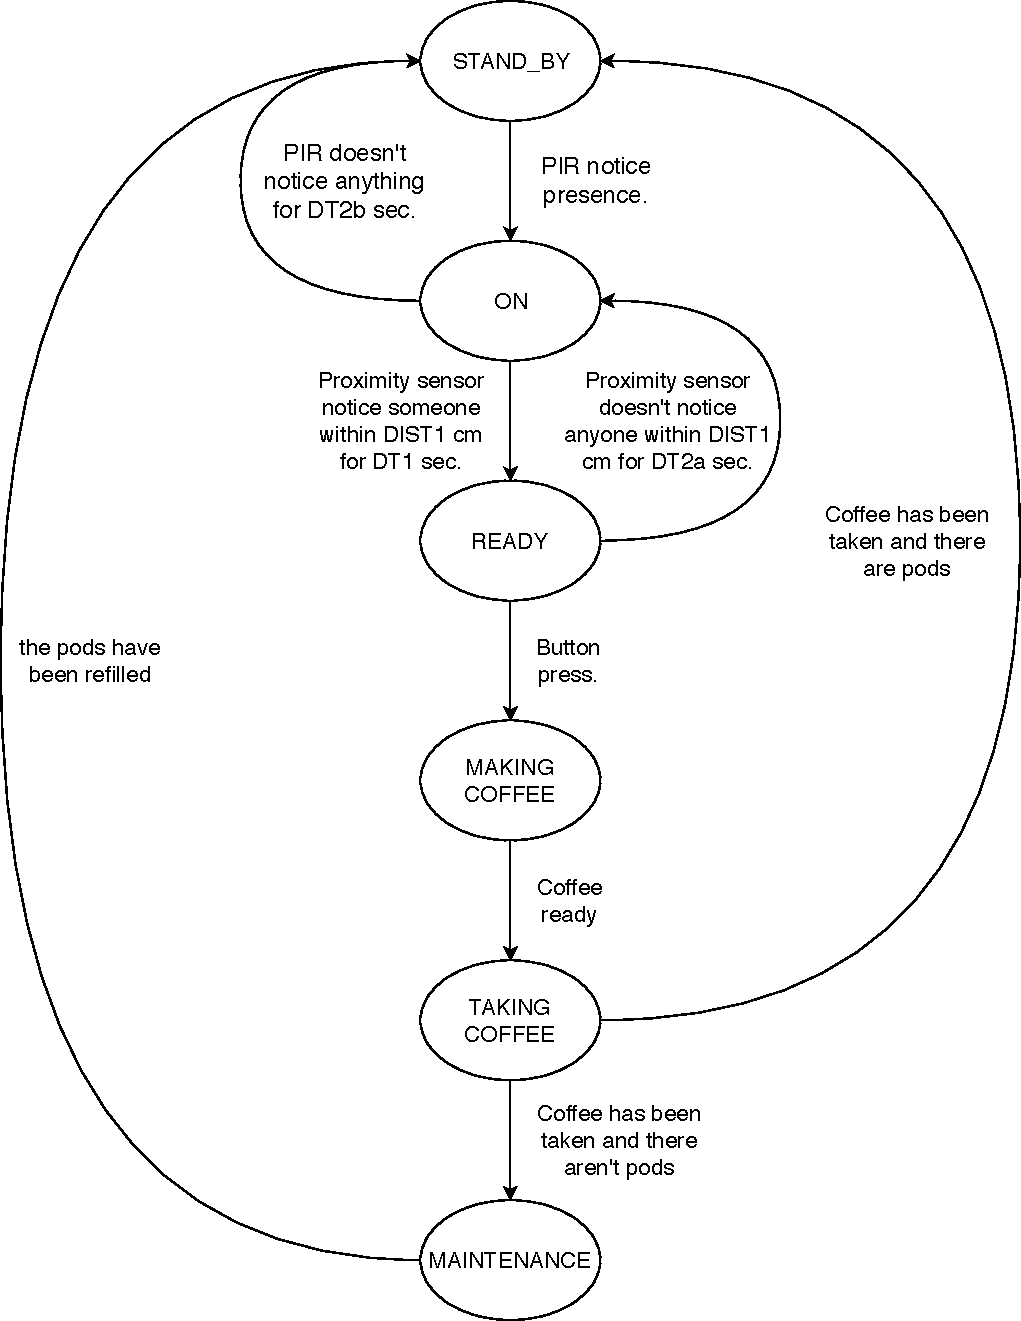
\includegraphics[scale=0.60]{res/pdf/general-fsm-crop.pdf} }
\end{center}
Questa FSM rappresenta il funzionamento generale della macchina, evidenziando i vari stati e le condizioni di transizione a un livello astratto e senza considerare quindi le variabili in gioco nel programma. Come si può evincere dallo schema, agli stati definiti nella consegna, sono stati aggiunti due ulteriori stati:
\begin{itemize}
	\item MAKING COFFEE
	\item TAKING COFFEE
\end{itemize}
Ci siamo presi la libertà di fare ciò perchè abbiamo considerato l'inserimento di questi due stati più esplicativo del funzionamento della macchina e perchè non abbiamo ritenuto che questo rendesse più facile o snaturasse l'intento del compito, ovvero l'apprendimento di utilizzo di un modello a task in un sistema integrato.

\subsection{State Switcher Task}
\vskip 0.3 cm
\begin{center}
\centering { 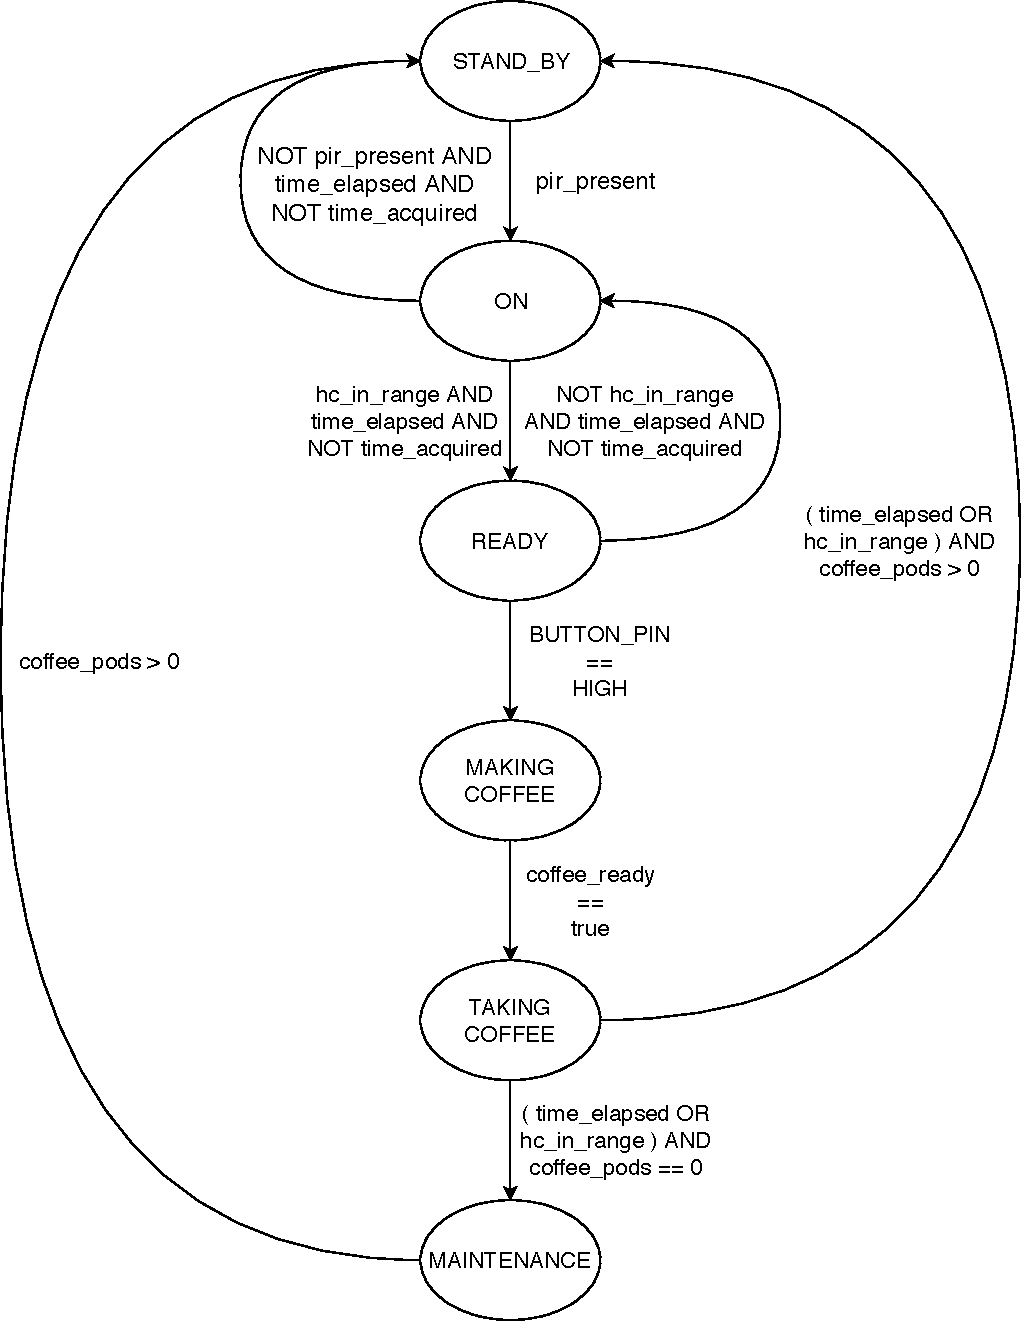
\includegraphics[scale=0.60]{res/pdf/stateswitcher-fsm-crop.pdf} \par }
\end{center}
E' di seguito inserito lo schema della FSM relativa al vero e proprio task "State Switcher". La descrizione di questa non si discosta dalla precedente, ma invece mostra le condizioni di transizione da uno stato all'altro tramite le variabili presenti nel programma.

\subsection{Timer Task}
\vskip 0.3 cm
\begin{center}
\centering { 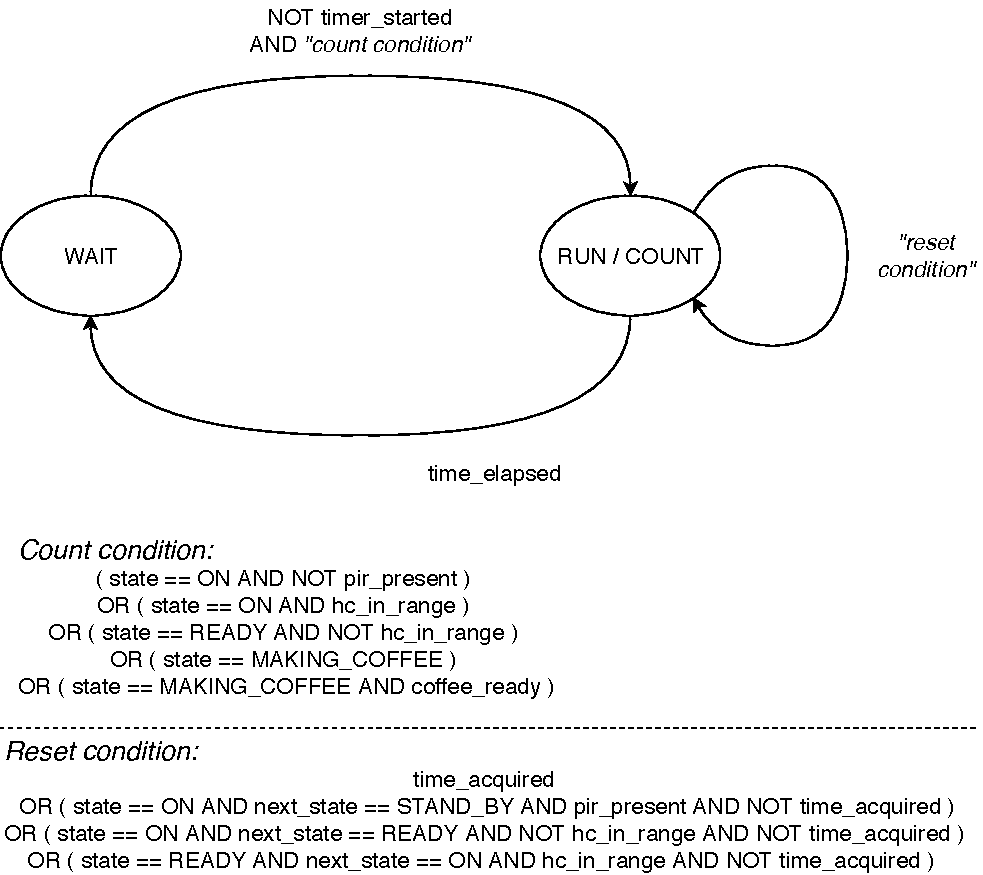
\includegraphics[scale=0.65]{res/pdf/timer-fsm-crop.pdf} \par }
\end{center}
La FSM del task Timer è molto semplice ma le condizioni di transizione tra i due stati sono varie. Per non appesantire troppo lo schema è stato scelto di non mostrare tutte le condizioni direttamente su questo, ma di inserire al loro posto un "riferimento" ad esse.

\newpage

%----------------------------------------------------------------------------------------
%	FRITZING
%----------------------------------------------------------------------------------------

\section{Fritzing}
\hfill
\begin{center}
\centering { 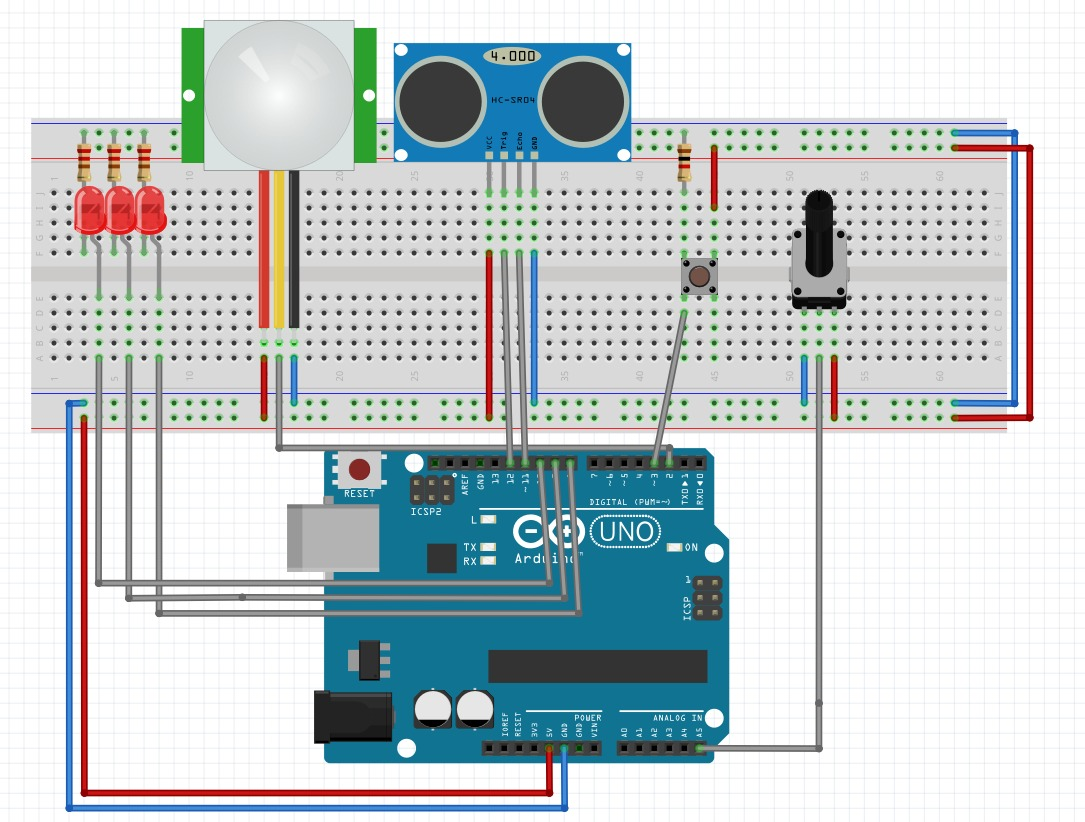
\includegraphics[rotate=90, width=\textwidth, center]{res/img/fritzing.jpeg} \par }
\end{center}

\newpage
%----------------------------------------------------------------------------------------


\end{document}